\clearpage\begingroup\SourceLeaf{73c}\HistoricalHead{68}{L}{PHYSIK. NACHLASS.}
\begin{center}[11.]\end{center}
\noindent{\small [S. 209]}
\begin{center}\textbf{Induktionsversuche.}\end{center}
\noindent\begin{tabular}{@{}l@{\quad}l@{}}
\multicolumn{1}{c}{\textls[120]{Widerstand}}&\multicolumn{1}{c}{\textls[120]{Erregungskraft}}\\[1ex]
\(1\) im Multiplikator.&\(e\) durch den ersten Erreger.\\
\(r\) im ersten Erreger, Induktionsrolle.&\(E\) durch den zweiten Erreger.\\
\(R\) im zweiten Erreger, Induktionsrad.&
\end{tabular}
\par\medskip\noindent\textls[120]{Wirkungen}
\[
\left.\begin{array}{l}a,\ b,\ c\\A,\ B,\ C\end{array}\right\}
\left.\begin{array}{l}\text{durch ersten}\\\text{durch zweiten}\end{array}\right\}
\text{Erreger}\left\{\begin{array}{l}\text{je nachdem der andere ausgeschlossen, oder}\\
\text{ohne oder mit Theilung in der Kette ist.}\end{array}\right.
\]
\clearpage\SourceLeaf{74}\HistoricalHead{69}{R}{BERECHNUNG MAGNETISCHER KRÄFTE.}
\indent Es ist dann
\[
\begin{alignedat}{2}
a&=\frac{e}{1+r}\qquad&A&=\frac{E}{1+R}\\[1ex]
b&=\frac{e}{1+r+R}&B&=\frac{E}{1+r+R}\\[1ex]
c&=\frac{eR}{r+R+rR}&C&=\frac{Er}{r+R+Rr}.
\end{alignedat}
\]
\noindent Ferner
\[
\begin{aligned}
aB+bA-aA=h\ \text{gesetzt, also}\ h&=\frac{eE}{(1+r)(1+R)(1+r+R)}\\
h&=bB-(a-b)(A-B)
\end{aligned}
\]
\[
\begin{alignedat}{2}
e&=\frac{abA}{h}\qquad&E&=\frac{ABa}{h}\\[1ex]
r&=\frac{a(A-B)}h&R&=\frac{A(a-b)}h\\[1ex]
1+r&=\frac{bA}h&1+R&=\frac{aB}h\\[1ex]
1+r+R&=\frac{aA}h.
\end{alignedat}
\]
\begin{center}Bedingungsgleichungen\end{center}
\[
\begin{aligned}
0&=abA+acA-abC-acB-bcA\\
0&=aAB+bAC-cAB-bAC-aBC
\end{aligned}
\]
\begin{center}oder\end{center}
\[
\begin{aligned}
ab(A-C)&=ch\\
AB(a-c)&=Ch
\end{aligned}
\]
\begin{center}oder einfacher\end{center}
\[
\begin{aligned}
0&=\frac Aa+\frac Bb+\frac Cc-\frac Ab-\frac Ac\\[1ex]
0&=\frac aA+\frac bB+\frac cC-\frac aB-\frac aC
\end{aligned}
\]
\begin{center}oder\end{center}
\[
\begin{aligned}
0&=\frac Aa-\frac{A-B}b-\frac{A-C}c\\[1ex]
0&=\frac aA-\frac{a-b}B-\frac{a-c}C.
\end{aligned}
\]
\noindent Am besten
\[
\frac Rr=\frac aA\frac{A-C}{a-c}=\frac Aa\frac{a-b}{A-B}=\frac{Bc}{Cb}.
\]
\begin{center}\rule{.23\textwidth}{.4pt}\end{center}
\noindent{\small [S. 210]}
\par\indent Die umstehenden Relationen stellen sich auch so dar.
\begin{center}(\(\mu\) Widerstand im Multiplicator)\end{center}
\[
\begin{aligned}
(1)&=\frac E{\mu+R}\\[1ex]
(2)&=\frac E{\mu+r+R}\\[1ex]
(3)&=\frac{Er}{\mu r+\mu R+rR}\\[1ex]
(4)&=(1)-(2)=\frac{Er}{(\mu+R)(\mu+r+R)}\\[1ex]
(5)&=(1)-(3)=\frac{E\mu R}{(\mu+R)(\mu r+\mu R+rR)}
\end{aligned}
\]
\[
\begin{aligned}
(6)&=\frac e{\mu+r}\\[1ex]
(7)&=\frac e{\mu+r+R}\\[1ex]
(8)&=\frac{eR}{\mu r+\mu R+rR}\\[1ex]
(9)&=(6)-(7)=\frac{eR}{(\mu+r)(\mu+r+R)}\\[1ex]
(10)&=(6)-(8)=\frac{e\mu r}{(\mu+r)(\mu r+\mu R+rR)}.
\end{aligned}
\]
\clearpage\SourceLeaf{75}\HistoricalHead{70}{L}{PHYSIK. NACHLASS.}
\begin{center}Bedingungsgleichungen.\end{center}
\[
\begin{aligned}
\frac{(1)\mathpunct{.}(1)}{(4)\mathpunct{.}(5)}&=\frac{(6)\mathpunct{.}(6)}{(9)\mathpunct{.}(10)}\\[1ex]
\frac{(1)\mathpunct{.}(2)}{(3)\mathpunct{.}(5)}&=\frac{(6)\mathpunct{.}(7)}{(8)\mathpunct{.}(10)}\\[1ex]
\frac{(1)\mathpunct{.}(3)}{(2)\mathpunct{.}(4)}&=\frac{(6)\mathpunct{.}(8)}{(7)\mathpunct{.}(9)}
\end{aligned}
\]
\noindent oder
\[
\begin{aligned}
(1)\mathpunct{.}(1)\mathpunct{.}(9)\mathpunct{.}(10)&=(4)\mathpunct{.}(5)\mathpunct{.}(6)\mathpunct{.}(6)\\
(1)\mathpunct{.}(2)\mathpunct{.}(8)\mathpunct{.}(10)&=(3)\mathpunct{.}(5)\mathpunct{.}(6)\mathpunct{.}(7)\\
(1)\mathpunct{.}(3)\mathpunct{.}(7)\mathpunct{.}(9)&=(2)\mathpunct{.}(4)\mathpunct{.}(6)\mathpunct{.}(8)
\end{aligned}
\]
\[
\begin{aligned}
\frac Rr&=\frac{(1)\mathpunct{.}(9)}{(6)\mathpunct{.}(4)}=\frac{(5)\mathpunct{.}(6)}{(10)\mathpunct{.}(1)}=\frac{(2)\mathpunct{.}(8)}{(7)\mathpunct{.}(3)}\\[1ex]
\frac r\mu&=\frac{(4)\mathpunct{.}(8)}{(5)\mathpunct{.}(7)}=\frac{(3)\mathpunct{.}(4)\mathpunct{.}(6)}{(1)\mathpunct{.}(2)\mathpunct{.}(10)}=\frac{(1)\mathpunct{.}(3)\mathpunct{.}(9)}{(2)\mathpunct{.}(5)\mathpunct{.}(6)}\\[1ex]
\frac R\mu&=\frac{(3)\mathpunct{.}(9)}{(2)\mathpunct{.}(10)}=\frac{(1)\mathpunct{.}(8)\mathpunct{.}(9)}{(5)\mathpunct{.}(6)\mathpunct{.}(7)}=\frac{(4)\mathpunct{.}(6)\mathpunct{.}(8)}{(1)\mathpunct{.}(7)\mathpunct{.}(10)}
\end{aligned}
\]
\[
\begin{alignedat}{2}
\frac Er&=\frac{(1)\mathpunct{.}(2)}{(4)}\qquad&\frac eR&=\frac{(6)\mathpunct{.}(7)}{(9)}\\[1ex]
\frac ER&=\frac{(2)\mathpunct{.}(6)}{(9)}&\frac er&=\frac{(1)\mathpunct{.}(7)}{(4)}\\[1ex]
\frac{Er}{\mu R}&=\frac{(1)\mathpunct{.}(3)}{(5)}&\frac{eR}{\mu r}&=\frac{(6)\mathpunct{.}(8)}{(10)}\text{[\textsuperscript{*})]}.
\end{alignedat}
\]
\begingroup\renewcommand{\thefootnote}{}\footnotetext{[\textsuperscript{*}) In den hier von S. 210 des Handbuchs 19, Be abgedruckten Formeln ist in der Handschrift nur
bei der \textls[120]{ersten} Gleichung die Ziffer (1) in Klammern gesetzt.]}\endgroup
\bigskip\begin{center}\textbf{BEMERKUNGEN ZU [11.].}\end{center}
\begingroup\small
\indent In moderner Ausdrucksweise bedeuten \(e\) und \(E\) die durch die beiden Erreger erzeugten elektromotorischen
Kräfte, \(a,b,c\) sind die Stromstärken in den drei unterschiedenen Fällen. Die drei gemeinten
Schaltungen sind in der folgenden Skizze dargestellt:
\begingroup
\newcommand{\SevenCoil}{
\draw (0,0)
foreach \i in {1,...,7}{
.. controls ({.42*\i-.37},.25) and ({.42*\i},.25) .. ({.42*\i},0)
.. controls ({.42*\i},-.16) and ({.42*\i-.13},-.16) .. ({.42*\i-.13},0)
}
.. controls (2.81,.25) and (3.36,.25) .. (3.36,0);
}
\begin{center}
\begin{tikzpicture}[x=.85cm,y=.85cm,line width=.55pt]
\begin{scope}[shift={(0,3.4)}]\SevenCoil\end{scope}
\draw (0,3.4)--(0,1.6).. controls (0,.55) and (.5,0) .. (1.65,0)
.. controls (2.8,0) and (3.36,.55) .. (3.36,1.6)--(3.36,3.4);
\draw (1.65,0) circle[radius=.25];
\draw[->,>=stealth] (1.15,-.52)--(2.17,.56);
\node[above] at (1.68,3.53) {$e(r)$};\node[below right,inner sep=1pt] at (1.9,-.10) {$M(1)$};
\node[below] at (1.68,-.85) {$a=\dfrac{e}{1+r}$};
\begin{scope}[shift={(5.3,0)}]
\begin{scope}[shift={(0,3.4)}]\SevenCoil\end{scope}
\draw (0,3.4)
foreach \i in {1,...,8}{
.. controls (-.27,{3.4-.38*\i+.33}) and (-.27,{3.4-.38*\i}) .. (0,{3.4-.38*\i})
.. controls (.17,{3.4-.38*\i}) and (.17,{3.4-.38*\i+.13}) .. (0,{3.4-.38*\i+.13})
}
.. controls (-.27,.49) and (-.27,0) .. (0,0)--(1.65,0)
.. controls (2.8,0) and (3.36,.55) .. (3.36,1.6)--(3.36,3.4);
\draw (1.65,0) circle[radius=.25];
\draw[->,>=stealth] (1.15,-.52)--(2.17,.56);
\node[above] at (1.68,3.53) {$e(r)$};\node[right,inner sep=1pt] at (.26,1.8) {$E(R)$};
\node[below right,inner sep=1pt] at (1.9,-.10) {$M(1)$};
\node[below] at (1.68,-.85) {$b=\dfrac{e}{1+r+R}$};
\end{scope}
\begin{scope}[shift={(10.6,0)}]
\begin{scope}[shift={(0,3.4)}]\SevenCoil\end{scope}
\draw (0,3.4)--(0,1.6).. controls (0,.55) and (.5,0) .. (1.65,0)
.. controls (2.8,0) and (3.36,.55) .. (3.36,1.6)--(3.36,3.4);
\begin{scope}[shift={(0,1.8)}]\SevenCoil\end{scope}
\draw (1.65,0) circle[radius=.25];
\draw[->,>=stealth] (1.15,-.52)--(2.17,.56);
\node[above] at (1.68,3.53) {$e(r)$};\node[above] at (1.68,1.95) {$E(R)$};
\node[below right,inner sep=1pt] at (1.9,-.10) {$M(1)$};
\node[below] at (1.68,-.85) {$c=\dfrac{eR}{r+R+rR}$};
\end{scope}
\end{tikzpicture}
\end{center}
\endgroup

\noindent Ganz analog für \(A,B,C\), wo nur statt des ersten Erregers \((e)\) der zweite \((E)\) einzusetzen ist. Die ganze
Betrachtung dient offenbar der Prüfung des \textsc{Ohm}schen Gesetzes.
\par\raggedleft\textsc{Schaefer}.\par
\clearpage\endgroup\endgroup
